\section{Connectedness} 

  Now that we have seen many examples of topologies, and how one can construct them (e.g. with a metric, subspace, product, quotient), we can begin to talk about some properties of these spaces. The first one is \textit{connectedness}, which is analogous to a topological space being irreducible (e.g. not able to be separated into two smaller topological spaces). This is what we should keep in mind. 

\subsection{Connected Spaces} 

  Let's first go and concretely define what such a separation means.

  \begin{definition}[Separation]
    Let $X$ be a topological space. A \textbf{separation} of $X$ is a pair $U, V$ of disjoint nonempty open subsets of $X$ whose union is $X$. 
  \end{definition}

  \begin{definition}[Connected]
    The space $X$ is said to be \textbf{connected} if it satisfies the equivalent definitions 
    \begin{enumerate}
      \item there does not exist a separation of $X$. 
      \item the only subsets of $X$ that are clopen in $X$ are the empty set and $X$ itself. 
    \end{enumerate}
    and \textbf{disconnected} otherwise. 

    \begin{figure}[H]
      \centering 
      \begin{tikzpicture}[scale=1.2]
        % First diagram - disjoint sets
        \begin{scope}
          % Set A
          \draw[dashed, thick] plot [smooth cycle, tension=0.8] 
            coordinates {(-1.5,1) (-0.5,1.3) (0,0.5) (-0.8,-0.2) (-1.8,0.3)};
          \node at (-1,0.5) {$A$};
          
          % Set B
          \draw[dashed, thick] plot [smooth cycle, tension=0.8] 
            coordinates {(1,0) (1.8,0.2) (1.5,-0.8) (0.5,-0.6)};
          \node at (1.2,-0.3) {$B$};
        \end{scope}
        
        % Second diagram - sets with common boundary
        \begin{scope}[xshift=6cm]
          % Set A - upper portion with less rounding
          \draw[dashed, thick] 
            plot [smooth cycle, tension=0.0] 
            coordinates {(-1,1) (0,1.5) (1,1) (1,0) (-1,0)};
          \node at (0,0.7) {$A$};
          
          % Set B - lower portion with less rounding
          \draw[dashed, thick] 
            plot [smooth cycle, tension=0.0] 
            coordinates {(-1,0) (1,0) (0.5,-1) (-0.5,-1)};
          \node at (0,-0.5) {$B$};
        \end{scope}
      \end{tikzpicture}
      \caption{Two examples of spaces $X = A \sqcup B$ that are not connected. In the right, $A$ and $B$ overlap in their boundary but are not connected since they are open. } 
      \label{fig:separation}
    \end{figure}
  \end{definition}
  \begin{proof}
    If there exists a nontrivial clopen set $U \subsetneq X$, then $U \sqcup U^c$ is a separation of $X$. If $U \sqcup V$ is a separation, then $V = U^c$, and so $U$ is clopen. 
  \end{proof} 

  \begin{example}[Discrete and Indiscrete Topology]
    Any set $|S| > 1$ with the discrete topology is disconnected. All subsets in the indiscrete topology is connected.  
  \end{example}

  \begin{example}[Disconnected Sets can Share Limit Points] 
    Let $Y$ denote the subspace $[-1,0) \cup (0,1]$ of $\mathbb{R}$. Each of the sets $[-1,0)$ and $(0,1]$ is nonempty and open in $Y$ (but not in $\mathbb{R}$), so they form a separation of $Y$. Also, note that neither of these sets contains a limit point of the other (even though they have a common limit point $0$). 

    On the same note, the space $Y = (0,1) \times (0,1) \cup (1,2) \times (0,1) \subset \mathbb{R}^2$ has the clear separation 
    \begin{equation}
      (0, 1) \times (0, 1) \text{ and } (1, 2) \times (0, 1)
    \end{equation}

    \begin{figure}[H]
      \centering 
      \begin{tikzpicture}[scale=1.5]
        \draw[dashed] (0,0) rectangle (2,1);
        \draw[dashed] (1,1)--(1,0);
      \end{tikzpicture}
      \caption{We can visualize the separation of $Y$ as such. } 
      \label{fig:separation_of_rectangle}
    \end{figure}
    Note that the dashed line is not in $Y$. Even though the dashed line contains limit points of both the left and right subset of $Y$, this does not matter. 
  \end{example} 

  Note that connectedness is a property of a topological space. Often we will talk about connected subsets $S \subset X$, but this should be taken to mean that $S$ is connected with respect to the subspace topology endowed from $X$. Now let's go to our standard space and see which sets are connected. For this, we will need to visit a bit of real analysis and recall the least upper bound property of the reals. 

  \begin{theorem}[Convex Subsets of Reals are Connected]
    $Y$ is a convex\footnote{We can define it with the order by saying that an ordered set $Y$ is convex is given $a, b \in Y$ and a $c$ s.t. $a < c < b$, then $c \in Y$.} subset of $\mathbb{R}$ iff $Y$ is connected. 
  \end{theorem}
  \begin{proof}
    We prove by contradiction. Suppose $Y = A \cup B$ disjoint, nonempty, and open in the subspace topology. Choose $a \in A, b \in B$ and WLOG let $a < b$. Now let 
    \begin{equation}
      A_0 = A \cap [a, b], \qquad B_0 = B \cap [a, b]
    \end{equation}
    Then $A_0 \sqcup A_0 = [a, b]$ with $A_0, B_0$ open in the subspace topology in $[a, b]$. Furthermore, $A_0$ is bounded above so it has a least upper bound. Let $c = \sup{A_0}$. 
    \begin{enumerate}
      \item If $c \in A_0$, by $A_0$ open there exists a right interval $[c, c + \epsilon) \subset A_0 \implies c + \frac{\epsilon}{2} \in A_0$, which means $c$ is not an upper bound. 
      \item If $c \in B_0$, by $B_0$ open there exists a left interval $(c - \epsilon, c] \subset B_0 \implies c - \frac{\epsilon}{2} \in B_0 $, which means $c$ is not least. 
    \end{enumerate}
  \end{proof}
  
  Note that this is sort of similar to proving how if vectors $v_1, \ldots, v_n$ are linearly independent, then 
  \begin{equation}
    a_1 v_1 + \ldots + a_n v_n = 0 \iff a_1 = a_2 = \ldots = a_n = 0
  \end{equation}
  This is generally, the method to prove whether a space is connected. 

  \begin{corollary}
    $\mathbb{R}$ with the standard topology is connected. Furthermore all intervals and rays are connected subsets of $\mathbb{R}$. 
  \end{corollary} 

  \begin{example}[More Topologies on Real Lines]
    Note that 
    \begin{enumerate}
      \item $\mathbb{R}$ with the lower limit topology is disconnected, since $(-\infty, a) \sqcup [a, +\infty)$ is a separation. 
      \item $\mathbb{R}$ with the finite complement topology is connected. In this case, no two open sets are even disjoint, and so this space is very very connected. 
    \end{enumerate}
  \end{example}

  \begin{example}[Dense Disconnected Sets]
    The rationals $\mathbb{Q} \subset \mathbb{R}$ are not connected since given any irrational number $r$, we can write $Y$ as the union of sets
    \begin{equation}
      Y \cap (-\infty, r), \; Y \cap (r, +\infty)
    \end{equation}
    which are open in the subspace topology. 
  \end{example}

  Great, so to prove whether subspaces are connected, we can just think of the subspace topology. But warning: note that since a separation of $Y \subset X$ is a pair of nonempty open sets $A, B \subset Y$ s.t. $A \sqcup B = Y$, since by openness $A = U \cap Y, B = V \cap Y$ for $U, V$ open in $X$, it may be the case that the larger open sets $U, V$ actually have an intersection. 

  \begin{figure}[H]
    \centering 
      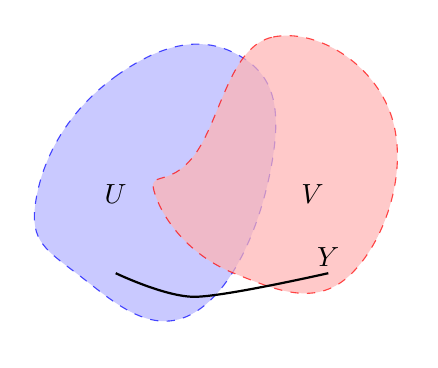
\begin{tikzpicture}
        % First blob using random smooth closed curve
        \draw[dashed, blue, fill=blue!30, opacity=0.7] 
          plot[smooth cycle, tension=0.8] 
          coordinates {(0,0) (1,1.5) (2.5,1.8) (3,0.5) (2,-1.5) (0.5,-1)};

        % Second blob using random smooth closed curve
        \draw[dashed, red, fill=red!30, opacity=0.7] 
          plot[smooth cycle, tension=0.8] 
          coordinates {(2,0.5) (3,2) (4.5,1) (4,-1) (2.5,-1) (1.5,0)};

        % Optional: Add labels
        \node at (1,0) {$U$};
        \node at (3.5,0) {$V$}; 
        \node at (3.7,-0.8) {$Y$}; 
        
        % Horizontal curve
        \draw[thick, -] 
          plot[smooth] coordinates {(1,-1) (2,-1.3) (3.7,-1.0)};
      \end{tikzpicture}
    \caption{We can see that there is a separation of $A = U \cap Y, B = V \cap Y$ of $Y$, but $U$ and $V$ do intersect.} 
  \end{figure}

  Therefore, we cannot rely on the topology on $X$ to deduce connectivity on $Y$. However, there is another simpler lemma that checks for connectivity of subspaces. 

  \begin{lemma}[Closures of One Separated Component is Disjoint from Other]
    If $A, B$ is a separation of subspace $Y \subset X$, then $A^\prime \cap B = \emptyset$ and $A \cap B^\prime = \emptyset$. It immediately follows that 
    \begin{equation}
      \overline{A} \cap B = A \cap \overline{B} = \emptyset
    \end{equation}
  \end{lemma}
  \begin{proof}
    If $A, B$ is a separation, then $A \subset U, B \subset V$ for $U, V$ open in $X$, and $A \cap V = \emptyset, B \cap U = \emptyset$. So points on $B \subset V$ are not limit points of $A$, and same with points on $A$. 
  \end{proof} 

  \begin{lemma}[Connected Subsets Must be Completely Contained in a Separated Component]
    If the sets $C$ and $D$ form a separation of $X$, and if $Y$ is a connected subset of $X$, then $Y$ lies entirely within either $C$ or $D$. 
  \end{lemma}
  \begin{proof}
    We can see that $A = C \cap Y$ and $B = D \cap Y$are open in the subspace topology of $Y$. So $A \cap B = \emptyset$ and $A \cap B = Y$, so either $Y = A$ or $Y = B$. 
  \end{proof}

  Now so far, we have treated connectedness as a property of a space, but we may extend this to talk about whether \textit{points} are connected. Essentially, we want to describe connectedness as an equivalence relation between points. The most nontrivial property is transitivity, which will be established in the following theorem. 

  \begin{theorem}[Points are Connected in a Connected Space]
    Let $X$ be a topological space. Then $X$ is connected iff $\forall x, y \in X$, $\exists$ a connected subspace $A$ s.t. $x, y \in A$. 
  \end{theorem}
  \begin{proof}
    We prove bidirectionally. 
    \begin{enumerate}
      \item $(\rightarrow)$. Take $A = X$. 
      \item $(\leftarrow)$. Let $X = U \cup V$ with $U \cap V = \emptyset$, both nonempty and open. Take $x \in U, y \in V$. So $\exists$ connected $A \subset X$ s.t. $x, y \in A$. But then either $A \subset U$ or $A \subset V$ from the lemma above. Therefore, $X$ is connected by contradiction. 
    \end{enumerate}
  \end{proof}

  Now, we can define connected components as an equivalence class. 

  \begin{corollary}[Connectedness is an Equivalence Relation]
    Let $x \sim_c y$ iff $\exists$ a connected subspace $A \subset X$ s.t. $x, y \in A$. 
  \end{corollary}
  \begin{proof}
    We prove the 3 properties. 
    \begin{enumerate}
      \item \textit{Reflexive}. $x \sim_c x$ clearly since $A = \{x\}$, which is connected. 
      \item \textit{Symmetric}. Let $x \sim_c y$. Then there exists connected subspace $A$ containing both $x, y$, i.e. containing $y, x$, and so $y \sim_c y$. 
      \item \textit{Transitive}. Let $x \sim_c y, y \sim_c z$. Then there exists connected subspaces $A \ni x, y$ and $B \ni y, z$. Since $y \in A \cap B$, $A \cup B$ is also a connected subspace containing $x, z$, and so $x \sim_c z$. 
    \end{enumerate}
  \end{proof}

  \begin{definition}[Connected Components]
    Given a topological space $X$, the equivalence classes under $\sim_c$ are called \textbf{connected components} of $X$. 
  \end{definition}

  With the equivalence class interpretation, it will be much easier to prove many properties. 

\subsection{Constructing Connected Spaces}

  We have proved some pretty basic results, and just like how we have talked about building new topologies from old ones, we can talk about how to build new connected spaces from old connected spaces. The three that we will mention are the unions, limit point extensions, and products. 

\subsubsection{Extensions}

  \begin{theorem}[Conditions for Union of Connected Spaces to be Connected]
    Suppose $A_\alpha \subset X$ are connected subspaces of $X$ s.t. $\forall \alpha, \beta$, $A_\alpha \cap A_\beta = \emptyset$. Then $\cup_\alpha A_\alpha$ is connected. 

  \begin{figure}[H]
    \centering 
    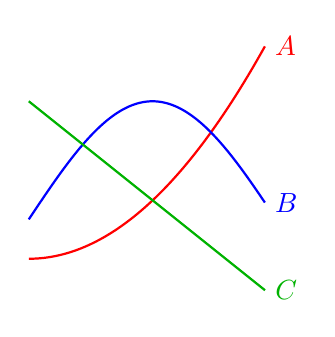
\begin{tikzpicture}
      % Curve A (parabola)
      \draw[thick, red, domain=0:3, samples=100] 
        plot (\x, {0.3*\x*\x - 2}) 
        node[right] {$A$};
        
      % Curve B (sine wave)
      \draw[thick, blue, domain=0:3, samples=100] 
        plot (\x, {1.5*sin(\x r) - 1.5}) 
        node[right] {$B$};
        
      % Curve C (line)
      \draw[thick, green!70!black, domain=0:3] 
        plot (\x, {-0.8*\x}) 
        node[right] {$C$};
    \end{tikzpicture}
    \caption{We can see that the connected subspaces $A, B, C \subset \mathbb{R}^2$ intersect pairwise at a point. Therefore their unions is connected. } 
  \end{figure}

  \end{theorem}
  \begin{proof}
    Let $A = \cup_\alpha A_\alpha$. Suppose $A = C \sqcup D$ with $C, D$ both open in subspace topology, so $C = A \cap U, D = A \cap V$ for $X$-open sets $U, V$. Each $A_\alpha$ is either in $C$ or $D$, since otherwise I can create a separation. But if $A_\alpha \subset C$ or $A_\alpha \subset D$, then this is impossible since they intersect at one point at least. So either all $A_\alpha \subset C$ or all $A_\alpha \subset D$. 
  \end{proof} 

  \begin{theorem}[Connected Sets plus Some/All Limit Points are Connected]
    Let $A$ be a connected subset of $X$. If $A \subset B \subset \bar{A}$, then $B$ is also connected. 
  \end{theorem}
  \begin{proof}
    Assume $B = C \cup D$ is a separation of $B \implies A$ must lie entirely within $C$ or $D$. Without loss of generality, suppose $A \subset C$, which implies that $\bar{A} \subset \bar{C}$. Since $\bar{C}$ and $D$ are disjoint, $B$ cannot intersect $D \implies D = \emptyset$, a contradiction. Therefore, there exists no separation of $B$. 
  \end{proof}

  \begin{theorem}[Products of Connected Spaces are Connected]
    Given connected topological spaces $X_\alpha$ with $\alpha \in J$, the Cartesian product 
    \begin{equation}
      \prod_{\alpha \in J} X_\alpha
    \end{equation}
    under the product topology is connected.\footnote{But for infinite products, it is not necessarily connected under the box topology} 

    \begin{figure}[H]
      \centering 
      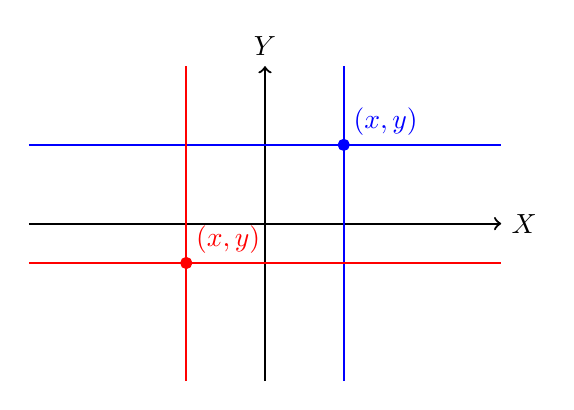
\begin{tikzpicture}
        % Coordinate axes
        \draw[thick, ->] (-3,0) -- (3,0) node[right] {$X$};
        \draw[thick, ->] (0,-2) -- (0,2) node[above] {$Y$};
        
        % Grid lines through point (1,1)
        \draw[blue, thick] (-3,1) -- (3,1) node[right] {};
        \draw[blue, thick] (1,-2) -- (1,2) node[above] {};

        \draw[red, thick] (-3,-0.5) -- (3,-0.5) node[right] {};
        \draw[red, thick] (-1,-2) -- (-1,2) node[above] {};
        
        % Mark the point (1,1)
        \filldraw[blue] (1,1) circle (2pt) node[anchor=south west] {$(x, y)$};
        \filldraw[red] (-1,-0.5) circle (2pt) node[anchor=south west] {$(x, y)$};
      \end{tikzpicture}
      \caption{You can see that any two $T_{x \times y}$ have a nontrivial intersection by construction. This is why we need the $+$ shape.} 
    \end{figure}
  \end{theorem}
  \begin{proof}
    We will prove for the finite product case. Given $(x, y) \in X \times Y$, let us define the space 
    \begin{equation}
      T_{x \times y} \coloneqq (\{x\} \times Y) \cup (X \times \{y\})
    \end{equation}
    where both of the components are connected (since they are homeomorphic to $Y$ and $X$, respectively). We know that $T_{x \times y}$ is connected since it's a union of connected space with nontrivial intersection $(x, y)$, and using the same lemma, the arbitrary union over all points in $X \times Y$ is connected. 
    \begin{equation}
      \bigcup_{(x, y) \in X \times Y} T_{x \times y} = X \times Y
    \end{equation}
    is connected. 
  \end{proof}

  \begin{example}[Connected Components in $\mathbb{R}^n$]
    $\mathbb{R}^n$ is connected, since it's a finite product of $\mathbb{R}$, which we proved was connected. Similarly, all $n$-cells of form $\prod_{i=1}^n (a_i, b_i)$ are also connected as a product of convex sets. 
  \end{example} 

  We will expand on this to prove some already intuitive results. 

  \begin{theorem}
    If $n > 1$, then for any $a \in \mathbb{R}^n$, $\mathbb{R}^n \setminus \{a\}$ is connected. 
  \end{theorem}
  \begin{proof}
    Let $U = \{x \in \mathbb{R}^n \mid x_n > a_n\}$ and $V = \{x \in \mathbb{R}^n \mid x_n < a_n\}$. These are connected since they are of form $\mathbb{R}^{n-1} \times (a, b)$. Now let 
    \begin{align}
      U^\prime & = U \cup \{x \in \mathbb{R}^n \mid x_n = a_n\} \setminus \{a\} \\
      V^\prime & = V \cup \{x \in \mathbb{R}^n \mid x_n = a_n\} \setminus \{a\} 
    \end{align}
    Note that $U^\prime, V^\prime$ are the $U, V$ plus some of its limit points, and so they are connected as well. So $U^\prime \cup V^\prime = \mathbb{R}^n \setminus \{a\}$ connected since they have a nontrivial intersection. 
  \end{proof}

  \begin{corollary}
    $\mathbb{R} \not\cong \mathbb{R}^n$ for $n > 1$. 
  \end{corollary}

\subsubsection{Images of Connected Spaces Under Functions}

  \begin{theorem}[Continuous Images of Connected Spaces are Connected]
    If $X$ is aconnected and $f: X \rightarrow Y$ is continuous, then $f(X)$ is a connected subspace of $Y$. 
  \end{theorem}
  \begin{proof}
    Let $f: X \longrightarrow Y$ be a continuous map, and let $X$ be connected. We wish to prove that the image set $Z = f(X)$ is also connected. Let us denote the restriction of $f$ to $Z$ as
    \begin{equation}
      \Tilde{f}: X \longrightarrow Z
    \end{equation}
    which is continuous and surjective. We prove by contradiction. Assume that $Z = A \cup B$ is a separation of $Z$ into 2 disjoint nonempty open sets. Then, $\Tilde{f}^{-1} (A)$ and $\Tilde{f}^{-1}(B)$ are disjoint open sets whose union is $X \implies \Tilde{f}^{-1} (A) \cup \Tilde{f}^{-1}(B)$ form a separation of $X$. This contradicts the hypothesis that $X$ is connected $\implies Z$ is connected.  
  \end{proof} 

  This establishes the fact that homeomorphisms preserve connectedness, and so connectedness is a topological property.  

  \begin{corollary}[Connectedness is a Topological Property]
    If $X \cong Y$, then $X$ connected iff $Y$ connected. 
  \end{corollary}

  Therefore, connectedness is a good way to prove that two spaces are not homeomorphic, whether it is by assuming a homeomorphism itself or taking the restriction of a homeomorphism with one or more points taken off the domain. 

  \begin{example}[Intervals of Endpoints $0$ and $1$]
    We claim that $(0, 1)$, $[0, 1)$, and $[0, 1]$ are all pairwise not homeomorphic. 
  \end{example}

  \begin{corollary}[Quotient Spaces]
    If $X$ is connected, then any quotient space of $X$ is connected. 
  \end{corollary}

  \begin{example}
    For $n \geq 1$, $S^n$ and $\mathbb{RP}^n$ is connected. 
  \end{example}

  Finally, we conclude with a theorem often seen in calculus, but is really a theorem in topology, since it only relies on continuity rather than derivatives, like the MVT. 

  \begin{theorem}[Intermediate Value Theorem]
    Let $f: X \longrightarrow Y$ be a continuous map of the connected space $X$ into the ordered set $Y$, with the order topology. Given $a, b \in X$ and $r \in Y$ such that $f(a)<r<f(b)$, then there exists a point $c \in X$ such that $f(c) = r$. 
  \end{theorem}
  \begin{proof}
    Assuming the hypothesis, the sets 
    \begin{equation}
      A \equiv f(X) \cap (-\infty, r), \; B \equiv f(X) \cap (r, +\infty)
    \end{equation}
    are disjoint. They are also nonempty since 
    \begin{equation}
      f(a) \in A, \; f(b) \in B
    \end{equation}
    $A$ and $B$ are open since they are the intersection of open sets. Now, assume that there exists no point $c \in X$ such that $f(c) = r$. Then, 
    \begin{equation}
      f(X) = A \cup B
    \end{equation}
    would define a separation of $X$, contradicting the fact that the image of a connected space under a continuous map must be connected. Therefore, $c$ exists. 
  \end{proof}  

\subsection{Path Connectedness} 

  Now we will be talking about a stronger form called path connectedness. Unlike connectedness---where we began with the topological definition and then claimed that the connected components form an equivalence class---we will introduce path connectedness as an equivalence class from the start. Note that connectedness is about open sets rather than paths. 

  \begin{definition}[Path]
    A \textbf{path} from $x \in X$ to $y \in X$ is a continuous function $f: [a, b] \subset \mathbb{R} \rightarrow X$\footnote{Note that we can just reparameterize the path to any other starting and end points with the homeomorphism $[a, b] \cong [c, d$.} s.t. $f(a) = x, f(b) = y$, and $[a, b]$ is endowed with the Euclidean topology.\footnote{So far, we've been pretty agnostic of topologies in definitions, but here we mention a very specific topology.} Two points $x, y$ are said to be \textbf{path connected}, denoted $x \sim_p y$, if there exists a path from $x$ to $y$, i.e. $f(0) = x, f(1) = y$.
  \end{definition} 

  \begin{lemma}[Path Components are Equivalence Classes]
    $\sim_p$ is an equivalence relation, and the equivalence classes formed by $\sim_p$ on topological space $X$ are called \textbf{path components}.  
  \end{lemma}
  \begin{proof}
    We prove the 3 properties. 
    \begin{enumerate}
      \item \textit{Reflexive}. $x \sim_p x$ since we can choose the constant function $f: t \mapsto x$.  
      \item \textit{Symmetric}. Let $x \sim_p y$. Then there exists a continuous $f: [0, 1] \rightarrow X$ s.t. $f(0) = x, f(1) = y$. We can choose the continuous function $g = f \circ h$, where $h(x) = 1 - x$ is continous connecting $y$ to $x$. 
      \item \textit{Transitive}. Let $x \sim_p y$ and $y \sim_p z$. then by the pasting lemma, the overlapping set $\{y\}$ is closed and so we can define the continuous function 
      \begin{equation}
        (f \ast g)(t) \coloneqq \begin{cases} 
          f(2t) & t \in [0, 1/2] \\
          g(2t - 1) & t \in [1/2, 1] 
        \end{cases} 
      \end{equation}
      which is a path from $x$ to $z$. 

      \begin{figure}[H]
        \centering 
        \begin{tikzpicture}
          % Define styles for the endpoints
          \tikzset{
            endpoint/.style={
              circle,
              fill=black,
              inner sep=0pt,
              minimum size=4pt
            }
          }
          
          % First curved line with endpoints
          \node[endpoint] (A) at (1,0) {};
          \node[endpoint] (B) at (4,2) {};
          \draw (A) to[out=50, in=210] (B);
          
          % Second curved line with endpoints
          \node[endpoint] (C) at (4,2) {};
          \node[endpoint] (D) at (6,1) {};
          \draw (C) to[out=20, in=200] (D);
          
          % Labels for the endpoints (optional)
          \node[below left] at (A) {$x$};
          \node[below right] at (B) {$y$};
          \node[above right] at (D) {$z$};
        \end{tikzpicture}
        \caption{W:}
      \end{figure}
    \end{enumerate}
  \end{proof}

  \begin{definition}[Path Connected Space] 
     A topological space $X$ is said to be \textbf{path connected} for every pair of points $x, y \in X$, $x \sim_p y$. 
  \end{definition}

  It seems that path connectedness is conceptually easier to deal with, and we might ask if one implies the other. 

  \begin{theorem}[Path Connectedness implies Connectedness]
    $X$ is path connected $\implies X$ is connected. That is, each path component is contained in a connected component. 

    \begin{figure}[H]
      \centering 
      \begin{tikzpicture}[scale=0.5]
        \draw[dashed] (5,1) circle (2);
        \draw[dashed] (0,0) circle (2);
        \node at (-1,-1) {$C$};
        \node at (6,2) {$D$};
        \draw plot [smooth] coordinates {(0,0) (2,1.5) (4.5,2)};
        \draw[fill] (0,0) circle (0.05);
        \draw[fill] (4.5,2) circle (0.05);
        \node at (-4,1) {$X = C \cup D$};
      \end{tikzpicture}
      \caption{Visually if two spaces are not connected, it doesn't seem like it's path connected. }
      \label{fig:path_vs_reg_connectedness}
    \end{figure}
  \end{theorem}
  \begin{proof} 
    We can prove this in two ways. 
    \begin{enumerate}
      \item \textit{Directly}. if $x \sim_p y$, then $\exists$ a path $f: [0, 1] \rightarrow X$ s.t. $f(a) = x, f(b) = y$, and $\Im(f)$ is a connected subspace containing $x, y$. 

      \item \textit{Contrapositive}. $X$ not connected implies that there exists disjoint open subsets $C, D$ such that $C \cup D = X$. Assume that $X$ is path connected, i.e. there exists a continuous function $g: [0,1] \longrightarrow X$. Then the preimage of $C$ and $D$ in $X$ must be open sets $g^{-1} (C), g^{-1} (D) \subset [0,1]$ such that $g^{-1}(C) \cup g^{-1}(D) = [0,1]$. But this isn't possible since $[0,1]$ is connected, so by contradiction, $X$ is not path connected. The contrapositive of this statement results in the theorem. 
    \end{enumerate}
  \end{proof} 

  But is the converse true? Intuitively, it seems like it, but a pretty nasty construction of a counterexample is needed. 

  However, note that $X$ connected $\centernot\implies$ $X$ path connected. Note the following example. 

  \begin{example}[Topologist's Sine Curve]
    Let 
    \begin{equation}
      C = \{ (x, y) \in \mathbb{R}^2 \mid x > 0, y = \sin(1/x) \}
    \end{equation} 
    This is the image of a continuous function. It is both connected and path connected since $C \cong (0, +\infty)$. This is \textit{not} the topologist's sine curve. $C$ is not closed since it doesn't contain the limit points $\{(0, y) \mid 0 \leq y \leq 1 \}$ (in red), but if we do cake the closure $\overline{C} = C \cup (\{0\} \times [-1, 1])$, then \textit{this} is the TSC. 

    \begin{figure}[H]
      \centering 
      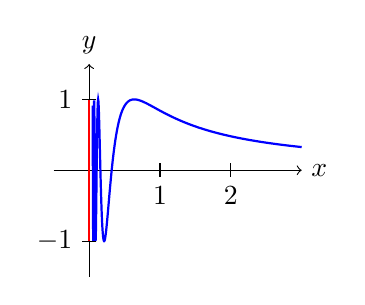
\begin{tikzpicture}[scale=0.9]
        % Draw the coordinate axes
        \draw[->] (-0.5,0) -- (3,0) node[right] {$x$};
        \draw[->] (0,-1.5) -- (0,1.5) node[above] {$y$};
        
        \draw[thick, blue, domain=0.05:3, samples=800, smooth, variable=\x] 
          plot ({\x}, {sin(1/\x r)});
        
        % Add vertical line at x=0
        \draw[dashed] (0,-1.5) -- (0,1.5);
        \draw[red, thick] (0,-1) -- (0,1);
        
        % Mark the x-axis and y-axis
        \foreach \x in {1,2}
          \draw (\x,0.1) -- (\x,-0.1) node[below] {$\x$};
        
        \foreach \y in {-1,1}
          \draw (0.1,\y) -- (-0.1,\y) node[left] {$\y$};
      \end{tikzpicture}
      \caption{Topologist's sine curve is the union of the image of the oscillating sine curve (blue) with its limit points (red).} 
      \label{fig:top_sine_curve}
    \end{figure}

    $\overline{C}$ is connected since the closure is the union of connected $C$ and some/all limit points of $C$. Now we claim that $\overline{C}$ is not path connected. Intuitively, given a point on $C$ and point on $C^\prime$, it must zig-zag infinitely many times, and thus cannot get to the red portion in time. Rigorously, suppose $f: [a, b] \rightarrow \overline{C}$ were a path from $(0, 0)$ to some $(x, y)$ with $x > 0$. $f^{-1} (\{x\} \times [-1, 1])$ is a closed subset of $[a, b]$ and thus has a max value; call it $c$. Now we take the restriction on $f: [c, b] \rightarrow \overline{C}$. Then 
    \begin{equation}
      f(c) \in C^\prime = \{0\} \times [-1, 1], \qquad f(t) \in C \; \forall t > c
    \end{equation} 
    Now reparaterize so that $c = 0, b = 1$. Then 
    \begin{equation}
      f(t) = \big( x(t), y(t) \big) = \big( x(t), \frac{1}{\sin{x(t)}} \big) 
    \end{equation}
    So we can find some sequence of numbers $t_n \rightarrow 0$ s.t. $y(t_n) = (-1)^n \implies \lim_{n \rightarrow +\infty} t_n = 0$ but $\lim_{n \rightarrow +\infty} y(t_n)$ does not exist, contradicting the fact that $f$ is continuous. 
  \end{example} 

  In general, mathematicians like path connectedness better since it makes our lives easier. We can more easily prove path connectedness by just building a path and it also implies connectedness.  

  \begin{example}[Euclidean Space]
    Let us take $\mathbb{R}^n$ and we claim the following. 
    \begin{enumerate}
      \item $\mathbb{R}^n$ is connected since given $x, y$, we can just draw $f(t) = (1 - t) x + ty$ for $t \in [0, 1]$, i.e. a straight line between them. 
      \item $\mathbb{R}^n \setminus \{0\}$ is path connected for $n > 1$ since we can draw a line, and if that line passes through the origin, i.e. $y = \lambda x$ for $lambda < 0$, then we choose $z \not\in \mathrm{span}(x)$ and choose the path $x \rightarrow z \rightarrow y$. 
      \item $\mathbb{R}^n \setminus S$ is path connected for any finite set $S$. 
    \end{enumerate}
  \end{example} 

  \begin{theorem}[Continuous Images of Path Connected Spaces as Path Connected]
    If $X$ is path connected and $f: X \rightarrow Y$ is continuous, then $f(X) \subset Y$ is path connected. 
  \end{theorem}
  \begin{proof}
    Given $y_1, y_2 \in f(X) \subset Y$, we choose $x_1, x_2$ s.t. $f(x_1) = y_1$ and $f(x_2) = y_2$. Then we choose a path $g$ from $x_1$ to $x_2$ since $X$ is path connected, and $f \circ g$ is a path from $y_1$ to $y_2$. 
  \end{proof}

  \begin{corollary}[Path Connectedness is a Topological Property]
    If $X \cong Y$, then $X$ path connected iff $Y$ path connected. 
  \end{corollary}

  \begin{corollary}[Quotients Path Connected Spaces are Path Connected]
    Any quotient of a path connected space is path connected. 
  \end{corollary}

  \begin{theorem}[Products of Path Connected Spaces]
    Any product of path connected spaces is path connected under the product topology.\footnote{Any only for finite products in the box topology.}
  \end{theorem}
  \begin{proof}
    Given $\prod_\alpha X_\alpha$ of path connected components $X_\alpha$, let $x = (x_\alpha), y = (y_\alpha)$ be its elements. Then for each $\alpha$, choose path $f_\alpha: [0, 1] \rightarrow X_\alpha$ with $f_\alpha (0) = x_\alpha$ and $f_\alpha (1) = y_\alpha$. Then by definition of product topology, the function 
    \begin{equation}
      f = \prod_\alpha f_\alpha : [0, 1] \rightarrow \prod_\alpha X_\alpha
    \end{equation}
    is continuous. 
  \end{proof}

  \begin{example}
    $\mathbb{R}^\omega$ is not even connected in the box topology. In fact it is horrifically disconnected. Let 
    \begin{equation}
      B \coloneqq \{x \in \mathbb{R}^\omega \mid |x_i| < R\}
    \end{equation}
    be the set of bounded sequences for some $R > 0$. We claim that $B$ is clopen in the box topology. Given $x \in \mathbb{R}^\omega$, let us define the open set
    \begin{equation}
      U_x = \prod (x_i - 1, x_i + 1) 
    \end{equation}
    If $x$ is bounded, then $x \in B$ and every element in $U_x$ is bounded $\implies U_x \subset B$. So $B$ is open. If $x$ is unbounded, then $x \in \mathbb{R}^\omega \setminus B$ and every element of $U_x$ is also unbounded $\implies U_x \subset \mathbb{R}^\omega \setminus B$. So $\mathbb{R}^\omega \setminus B$ is open and $B$ is closed. 
  \end{example}

\subsection{Local Connectedness and Path Connectedness}

  The property of local connectedness is also important for a space to possess. Roughly speaking, local connectivity means that each point has "arbitrarily small" neighborhoods that are connected. It is a property on small scales, i.e. for a property on open sets. 

  \begin{definition}[Locally (Path) Connected at a Point]
    A space $X$ is said to be \textbf{locally (path) connected at $x$} if for every neighborhood $U$ of $x$, there is a (path) connected open neighborhood $V$ of $x$ contained in $U$. If $X$ is locally (path) connected at all of its points, then $X$ is simply said to be \textbf{locally (path) connected}. 

    \begin{figure}[H]
      \centering 
      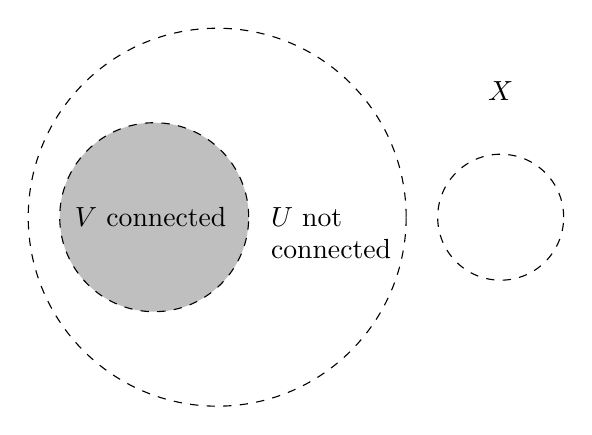
\begin{tikzpicture}[scale=0.8]
        \draw[fill] (-2,0) circle (0.05);
        \node[above] at (-2,0) {$x$};
        \draw[dashed] (-1.5,0) circle (3);
        \draw[dashed] (3,0) circle (1);
        \draw[dashed, fill=lightgray] (-2.5,0) circle (1.5);
        \node[left] at (-1.2,0) {$V$ connected};
        \node[right] at (-0.8,0) {$U$ not};
        \node[right] at (-0.8,-0.5) {connected};
        \node at (3,2) {$X$};
      \end{tikzpicture}
      \caption{Visually, in the space $X$, let $U$ be the union of the two open balls shown below. $U$ is clearly open, but not necessarily connected. However, we can form a  neighborhood $V$ of $x$ contained in $U$ such that $V$ is connected. }
      \label{fig:locally_connected}
    \end{figure}
  \end{definition} 

  \begin{example}[Euclidean Space]
    $\mathbb{R}^n$ plus any open sets in $\mathbb{R}^n$ is locally connected and locally path connected since open balls of any radius are path connected. 
  \end{example} 

  \begin{example}[Topologist's Sine Curve]
    The TSC is not locally connected.  

    \begin{figure}[H]
      \centering 
      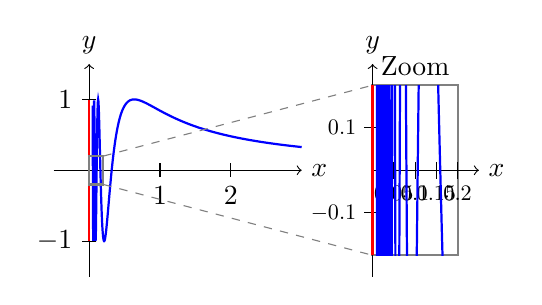
\begin{tikzpicture}[scale=0.9]
        % Draw the coordinate axes
        \draw[->] (-0.5,0) -- (3,0) node[right] {$x$};
        \draw[->] (0,-1.5) -- (0,1.5) node[above] {$y$};
        
        \draw[thick, blue, domain=0.05:3, samples=800, smooth, variable=\x] 
          plot ({\x}, {sin(1/\x r)});
        
        % Add vertical line at x=0
        \draw[dashed] (0,-1.5) -- (0,1.5);
        \draw[red, thick] (0,-1) -- (0,1);
        
        % Mark the x-axis and y-axis
        \foreach \x in {1,2}
          \draw (\x,0.1) -- (\x,-0.1) node[below] {$\x$};
        
        \foreach \y in {-1,1}
          \draw (0.1,\y) -- (-0.1,\y) node[left] {$\y$};
          
        % Add zoom box
        \draw[gray, thick] (0,-0.2) rectangle (0.2,0.2);
        
        % Draw the zoomed area
        \begin{scope}[shift={(4,0)}, scale=6]
          % Box outline
          \draw[gray, thick] (0,-0.2) rectangle (0.2,0.2);
          \node[above] at (0.1,0.2) {Zoom};
          
          % Axes for zoomed region
          \draw[->] (0,0) -- (0.25,0) node[right] {$x$};
          \draw[->] (0,-0.25) -- (0,0.25) node[above] {$y$};
          
          % Labels for x-axis in zoomed region
          \draw (0.05,0.02) -- (0.05,-0.02) node[below, scale=0.8] {$0.05$};
          \draw (0.1,0.02) -- (0.1,-0.02) node[below, scale=0.8] {$0.1$};
          \draw (0.15,0.02) -- (0.15,-0.02) node[below, scale=0.8] {$0.15$};
          \draw (0.2,0.02) -- (0.2,-0.02) node[below, scale=0.8] {$0.2$};
          
          % Labels for y-axis in zoomed region
          \draw (0.02,0.1) -- (-0.02,0.1) node[left, scale=0.8] {$0.1$};
          \draw (0.02,-0.1) -- (-0.02,-0.1) node[left, scale=0.8] {$-0.1$};
          
          % Clip the function in the zoomed area to stay within y = -0.2 to 0.2
          \begin{scope}
            \clip (0,-0.2) rectangle (0.2,0.2);
            \draw[thick, blue, domain=0.01:0.2, samples=1500, smooth, variable=\x] 
              plot ({\x}, {sin(1/\x r)});
          \end{scope}
          
          % Add vertical line at x=0 in zoomed region
          \draw[red, thick] (0,-0.2) -- (0,0.2);
        \end{scope}
        
        % Add connector lines between the boxes
        \draw[gray, dashed] (0.2,0.2) -- (4,1.2);
        \draw[gray, dashed] (0.2,-0.2) -- (4,-1.2);
      \end{tikzpicture}
      \caption{If we take a neighborhood around $(0, 0)$, we can see that the intersection of the image of a function with the open ball around the origin will consists of many almost-vertical lines that are not connected.} 
      \label{fig:top_sine_curve_2}
    \end{figure}
  \end{example}

  Even though local properties alone does not in general allow us to conclude about a global property, there are times when it does. 

  \begin{theorem}[LPC + C $\implies$ PC]
    If $X$ is locally path connected, connectedness $\iff$ path connectedness, i.e. the connected components and path connected components are the same. In other words, 
    \begin{equation}
      \text{Local Path Connectedness } + \text{ Connectedness} \implies \text{ Path Connectedness}
    \end{equation}
  \end{theorem} 

  Equivalently, $X$ is locally connected if there exists a basis for $X$ consisting of connected sets. Local connectedness and connectedness of a space are independent of each other. 

  \begin{theorem}[Open Components and Local (Path) Connectedness]
    Given space $X$, 
    \begin{enumerate}
      \item $X$ is locally connected iff its connected components are open. 
      \item $X$ is locally path connected if its path connected components are open. 
    \end{enumerate}
  \end{theorem}
  \begin{proof}
    For the first claim, we prove bidirectionally. 
    \begin{enumerate}
      \item $(\rightarrow)$ Suppose that $X$ is locally connected. Let $U$ be an open set of $X$ and let $C$ be a component of $U$. If $x$ is any point in $C$, by definition of local connectedness, there exists a connected neighborhood $V$ of $x$ fully contained in $U$. Since $V$ is connected, it must additionally lie completely within $C \implies C$ is open in $X$. 
      \item $(\leftarrow)$ Suppose that the components of open sets in $X$ are open. Given a point $x \in X$ and neighborhood $U$ of $x$, let $C$ be the component of $U$ containing $x$, which means that $C$ is connected. By hypothesis, the components of open sets are alsvo open, so $C$ is also open. Since an open, connected set $C$ exists for all $x \in X$, $X$ is locally connected. 
    \end{enumerate}
    For the second claim, we also prove bidirectionally. 
    \begin{enumerate}
      \item TBD. 
      \item TBD. 
    \end{enumerate}
  \end{proof}

\subsection{Homotopies}

  The concept of homotopies is dealt with in algebraic topology, but it is worthwhile to mention it now. 

  \begin{definition}[Homotopy]
    Two continuous paths from $x$ to $y$ in topological space $X$ is \textbf{homotopic} if one can be continuously "deformed" into the other, such a deformation being the \textbf{homotopy} between two functions. The set of linearly homotopic paths form a relation, and thus \textbf{homotopy classes} can be further defined. 
    \begin{figure}[H]
      \centering 
      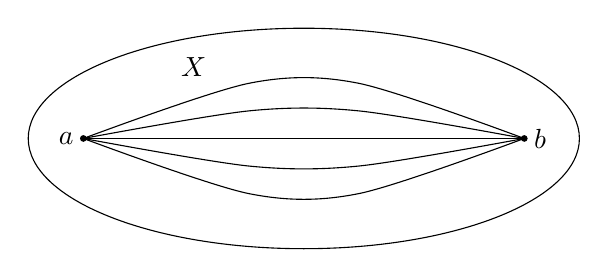
\begin{tikzpicture}[scale=0.7]
        \draw (0,0) ellipse (5 and 2);
        \draw[fill] (-4,0) circle (0.05);
        \draw[fill] (4,0) circle (0.05);
        \draw plot [smooth] coordinates {(-4,0) (-1,1) (1,1) (4,0)};
        \draw (-4,0)--(4,0);
        \draw plot [smooth] coordinates {(-4,0) (-1,0.5) (1,0.5) (4,0)};
        \draw plot [smooth] coordinates {(-4,0) (-1,-0.5) (1,-0.5) (4,0)};
        \draw plot [smooth] coordinates {(-4,0) (-1,-1) (1,-1) (4,0)};
        \node at (-2,1.3) {$X$};
        \node[left] at (-4,0) {$a$};
        \node[right] at (4,0) {$b$};
      \end{tikzpicture}
      \caption{Visually, the set of all the curves in the space $X$ as shown are in a single homotopy class.} 
      \label{fig:single_homotopy_class}
    \end{figure}
  \end{definition}

  It is clear that the space $X$ consists of a single homotopy class of curves from $a$ to $b$. However, a space may have an infinite number of such classes. 

  \begin{figure}[H]
    \centering 
    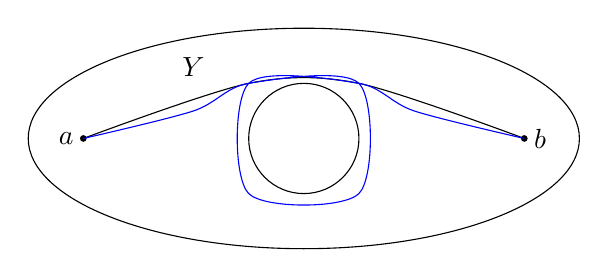
\begin{tikzpicture}[scale=0.7]
      \draw (0,0) ellipse (5 and 2);
      \draw[fill] (-4,0) circle (0.05);
      \draw[fill] (4,0) circle (0.05);
      \draw plot [smooth] coordinates {(-4,0) (-1,1) (1,1) (4,0)};
      \node[left] at (-4,0) {$a$};
      \node[right] at (4,0) {$b$};
      \draw (0,0) circle (1);
      \node at (-2,1.3) {$Y$};
      \draw[blue] plot [smooth] coordinates {(-4,0) (-2,0.5) (-1,1) (1,1) (1,-1) (-1,-1) (-1,1) (1,1) (2,0.5) (4,0)};
    \end{tikzpicture}
    \caption{Let us define the space $Y \equiv X \setminus C$ where $C$ is a circular region in $X$. Then, $Y$ has an infinite number of homotopy classes. We show two curves, that are in two different homotopy classes. }
    \label{fig:homotopy_class}
  \end{figure}

  \begin{definition}[Simply Connected Set]
    A \textbf{simply connected set} is a set such that all paths between any two given points are homotopic. That is, a simply connected set has one homotopy class. 
  \end{definition}


